%%% LaTeX Template: Article/Thesis/etc. with colored headings and special fonts
%%%
%%% Source: http://www.howtotex.com/

\documentclass[12pt]{article}


\usepackage{apuntes-estilo}
\usepackage{fancyhdr,lastpage}
\usepackage{color,colortbl}
\usepackage{verbatim}

\def\maketitle{

% Titulo 
 \makeatletter
 {\color{bl} \centering \huge \sc \textbf{
 Administración de Recursos \\ 
\large \vspace*{-8pt} \color{black} Guía básica de reconocimiento de recursos. 
 \vspace*{8pt} }\par}
 \makeatother


% Autor
 \makeatletter
 {\centering \small 
 	Departamento de Ingeniería de Computadoras \\
 	Facultad de Informática - Universidad Nacional del Comahue \\
 	\vspace{20pt} }
 \makeatother

}

% Custom headers and footers
\fancyhf{} % clear all header and footer fields
\fancypagestyle{plain}{\fancyhf{}}
  	\pagestyle{fancy}
 	\lhead{\footnotesize Reconocimiento de Recursos - Departamento de Ingeniería de Computadoras}
 	\rhead{\footnotesize \thepage\ }	% ''Page 1 of 2''

\def\ti#1#2{\texttt{#1} & #2 \\ }



\begin{document}

\thispagestyle{empty}
\maketitle
\setlength{\parindent}{0pt}

\section*{Introducción}

Un administrador de sistemas es quien gestiona los recursos de un sistema informático. 
Recordemos que la Administración de Sistemas es el conjunto de tareas necesarias para mantener
un computador en buenas condiciones de uso (agregar referencia al tutorial Introduccion).
Por lo tanto, una de las tareas elementales es conocer como
identificar y verificar el funcionamiento correcto de los recursos a gestionar.

En esta guía se describen procedimientos y programas que generalmente se utilizan
para identificar recursos, y verificar su estado.
Debido a la variedad del hardware existente hoy en día, este apunte no es
exhaustivo, pero plantea un método de identificación y monitoreo a partir de ejemplos. 
Cuando 
el recurso a administrar no este contemplado en esta guía el administrador deberá preguntarse e
investigar cuál es la forma de obtener información del recurso, y cómo observar su estado.

Los recursos detallados en este documento pueden referirse a :

\begin{itemize}
	\item recursos físicos, como por ejemplo una CPU (de los cuales nos interesa su reprensentación por software en el sistema operativo);
	\item o recursos netamente lógicos que no tienen una
contraparte física, como puede ser un proceso (programa en ejecución), una prioridad de ejecución, 
un sistema de archivos, etc. 
\end{itemize}



\section*{Identificando recursos}

Comenzaremos por identificar recursos físicos con un ejemplo, que nos permita
listar sus características y la forma en que 
se encuentra representado en el sistema operativo.
Un procedimiento sencillo de recordar, al momento de gestionar recursos, es pensar en la siguiente pregunta: \\
¿Qué programas nos permite obtener información acerca del dispositivo?. \\
Por ejemplo, si se necesita reconocer un dispositivo USB recientemente conectado, 
el administrador debe identificar el conjunto de comandos que le permita obtener información del recurso.
En este caso, la identificación de los programas útiles se resuelve casi 
de manera inmediata al realizar una búsqueda entre las páginas de manual de GNU/Linux: 

\colorbox{grey}{\parbox[t]{0.95\linewidth}{ \vspace*{0.5cm} { 
{\bf Ejemplo : Identificando un dispositivo USB} \\ \\
{\tt 
\$ man -k usb \\
lsusb (8)            - list USB devices\\
sane-find-scanner (1) - find SCSI and USB scanners and their device files\\
sisusb (4)           - SiS USB video driver\\
unetbootin (1)       - program to install Linux/BSD distributions to a partit...\\
update-usbids (8)    - download new version of the USB ID list\\
usb-devices (1)      - print USB device details\\
usb\_modeswitch (1)   - switch mode of ``multi-state'' USB devices\\
usb\_printerid (1)    - prints the ID of the printer on a USB port\\
usbip (8)            - manage USB/IP devices\\
usbipd (8)           - USB/IP server daemon\\
usbmuxd (1)          - iPhone/iPod Touch USB multiplex server daemon\\ \\
}
Observe que la primera y sexta línea de resultados tienen grandes chances 
de darnos la información que estamos buscando. Es importante remarcar que
siempre existen diversos modos de obtener la misma información. \\ 
\\
{\bf NOTA A PEGAR EN EL ESPEJO: ¡``{\tt man -k}'' es tu amigo! }
} \vspace*{0.5cm} } } 

Obviamente si el administrador no logra resultados investigando entre las 
páginas del manual de la máquina en cuestión, irá a Internet y haciendo la consulta
correcta ``list usb devices Linux'' ó ``listar usb en Linux'' (en 
muchos casos la búsqueda en idioma inglés devuelva más resultados que en español),  
muy probablemente obtendrá lo que busca entre los primeros resultados: 

\begin{center}
 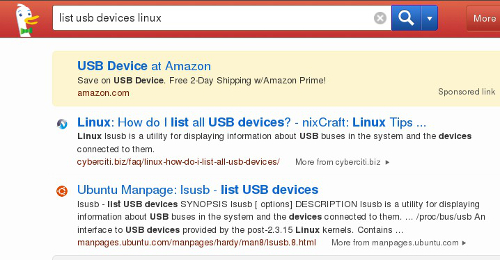
\includegraphics{lsusb.jpg}
\end{center}

Si no resuelve la pregunta de este modo, recurra a expertos en el tema, pero recuerde
intentar la identificación de recursos por sus propios medios al menos siguiendo los dos 
métodos anteriores, el administrador debe ser curioso e investigar, de otro modo puede 
obtener respuestas como esta: http://lmgtfy.com/?q=list+usb+devices+linux

\section*{Identificando el hardware}
En esta sección listaremos una serie de comandos clásicos para identificar recursos de
hardware dentro del sistema operativo. 

\subsection*{Aprendiendo a escuchar al kernel Linux}

Como sabemos, el kernel Linux es el primer elemento de software del sistema operativo 
que se carga luego del gestor de arranque, y es quien inicializa y toma control del hardware. 
El resto del sistema operativo que se carga a continuación de este, interactúa con el kernel 
cuando necesita utilizar el hardware con algún fin. 

A medida que el kernel Linux reconoce el hardware, tanto en el arranque como durante la 
operación normal del sistema al insertar y remover dispositivos de hardware 
en caliente (sin apagar la computadora), el kernel se comunica a través de mensajes para 
que el administrador tenga información acerca de lo que sucede. 

Estos mensajes son recolectados y guardados en archivos bitácora (logs) para su posterior 
revisión por parte de los administradores de sistemas. 
La información provistas por el kernel no se limita a reconocimiento del hardware, también 
provee información sobre el funcionamiento del mismo, y otros componentes lógicos que 
interactúan con el kernel. 
Es tarea del administrador leer la información que el kernel provee. 

En las secciones siguientes se proveen herramientas específicas para consultar el estado 
e información de dispositivos de hardware, sin embargo el administrador de sistemas debe
tener presente la información provista por el kernel en los archivos de bitácora y en su 
buffer (sección de memoria) temporal a modo de información complementaria; y en algunos 
casos, como único medio de información. Por este motivo, cada vez que se encuentre en el 
proceso de identificación de recursos, recuerde además de utilizar herramientas 
específicas, revisar los archivos de bitácora del sistema y el buffer temporal. 

\fcolorbox{black}{grey}{
\parbox[t]{1.0\linewidth}{ \vspace*{0.4cm}
En las distribuciones GNU/Linux el directorio {\bf \texttt{/var/log}} contiene diferentes 
archivos de bitácora donde distintos elementos del sistema reportan su actividad. En 
particular, es de interés el archivo {\bf \texttt{/var/log/messages}}, ya que es en dónde 
el kernel vuelca su información. 
\vspace*{0.4cm} } }


Cada línea en el archivo \texttt{/var/log/messages} consta de una estampilla de tiempo, 
el nombre del sistema, el componente del sistema operativo que reporta el mensaje y 
finalmente el mensaje. 

\fcolorbox{black}{grey}{
\parbox[t]{1.0\linewidth}{ \vspace*{0.4cm}
{\bf Ejemplo: mensajes del kernel Linux al conectar (en caliente) un módem 3g\\ }
\\ {\tt \scriptsize
Aug 17 12:00:47 m01 kernel: [490611.120188] usb 1-4: new high-speed USB device number 11 using ehci\_hcd\\
Aug 17 12:00:47 m01 kernel: [490611.253621] usb 1-4: New USB device found, idVendor=12d1, idProduct=14fe\\
Aug 17 12:00:47 m01 kernel: [490611.253625] usb 1-4: New USB device strings: Mfr=2, Product=1, SerialNumber=0\\
Aug 17 12:00:47 m01 kernel: [490611.253628] usb 1-4: Product: HUAWEI Mobile\\
Aug 17 12:00:47 m01 kernel: [490611.253630] usb 1-4: Manufacturer: HUAWEI\\
Aug 17 12:00:47 m01 kernel: [490611.255295] scsi12 : usb-storage 1-4:1.0\\
Aug 17 12:00:47 m01 kernel: [490611.255486] scsi13 : usb-storage 1-4:1.1\\
Aug 17 12:00:48 m01 mtp-probe: checking bus 1, device 11: ``/sys/devices/pci0000:00/0000:00:12.2/usb1/1-4''\\
Aug 17 12:00:48 m01 mtp-probe: bus: 1, device: 11 was not an MTP device\\
Aug 17 12:00:48 m01 kernel: [490612.253335] scsi 12:0:0:0: CD-ROM            HUAWEI   Mass Storage     2.31 PQ: 0 ANSI: 2\\
Aug 17 12:00:48 m01 kernel: [490612.253409] scsi 13:0:0:0: Direct-Access     HUAWEI   SD Storage       2.31 PQ: 0 ANSI: 2\\
Aug 17 12:00:49 m01 kernel: [490612.261977] sr1: scsi-1 drive\\
Aug 17 12:00:49 m01 kernel: [490612.265664] sr 12:0:0:0: Attached scsi generic sg2 type 5\\
Aug 17 12:00:49 m01 kernel: [490612.268493] sd 13:0:0:0: Attached scsi generic sg3 type 0\\
Aug 17 12:00:49 m01 kernel: [490612.271945] sd 13:0:0:0: [sdb] Attached SCSI removable disk\\
}
\vspace*{0.4cm} } }

Tenga en cuenta que no siempre observaremos la misma secuencia para un dispositivo en particular. 
Los mensajes del kernel dependen de la configuración del sistema.

\fcolorbox{black}{grey}{
\parbox[t]{1.0\linewidth}{ \vspace*{0.4cm}
{\bf Lo importante :} Incorporar el hábito de consultar los archivos de log e
identificar la información de interés para el recurso a identificar, o bien la ausencia de la misma.
\vspace*{0.4cm} } }

Además de los mensajes almacenados en el archivo \texttt{/var/log/message}, el kernel Linux posee un buffer 
(sección de memoria) en el que almacena temporalmente los mensajes que va emitiendo. Este buffer es 
finito y la información en él se va perdiendo a medida que nuevos mensajes son temporalmente guardados. Sirve para 
consultar los últimos mensajes emitidos, y no posee marcas de tiempo. Para ver la información contenida en el 
buffer utilizamos el comando \texttt{\textbf{dmesg}}. 

Por ejemplo cuando estamos tratando de reconocer la actividad del sistema al agregar y quitar 
dispositivos en caliente (hot plug en inglés), una secuencia clásica es :

\begin{enumerate}
	\item Ejecutar \texttt{dmesg} antes de conectar el dispositivo;
	\item Observar la última línea del buffer;
	\item Colocar el dispositivo;
	\item Volver a ejecutar \texttt{dmesg} para reconocer los nuevos mensajes producidos por el kernel.
\end{enumerate}


\subsection*{Información del CPU:}

Si miramos el resultado de \texttt{man -k cpu}, encontraremos muchos comandos probables, quizá 
uno de los más evidentes es \textbf{\texttt{lscpu}} cuya función es listar el contenido del archivo 
\texttt{/proc/cpuinfo} (normalmente los comandos ls{\textless}algo\textgreater  
\textbf{listan} información acerca de {\textless}algo\textgreater).

\colorbox{grey}{\parbox[t]{0.95\linewidth}{ \vspace*{0.5cm} { 
{\tt
\# lscpu \\
Architecture:          i686\\
CPU op-mode(s):        32-bit, 64-bit\\
Byte Order:            Little Endian\\
CPU(s):                2\\
On-line CPU(s) list:   0,1\\
Thread(s) per core:    1\\
Core(s) per socket:    2\\
Socket(s):             1\\
Vendor ID:             AuthenticAMD\\
CPU family:            16\\
Model:                 6\\
Stepping:              3\\
CPU MHz:               800.000\\
BogoMIPS:              5586.01\\
Virtualization:        AMD-V\\
L1d cache:             64K\\
L1i cache:             64K\\
L2 cache:              1024K\\
}
El mismo resultado se obtiene ejecutando \texttt{cat /proc/cpuinfo}
} \vspace*{0.5cm} } } 

El comando \textbf{\texttt{dmidecode}} tiene una sección ``Processor Information'' que muestra
información almacenada en el firmware de la placa base (SMBIOS) acerca de los componentes de 
hardware. 

A continuación mostramos un ejemplo de la salida de \texttt{dmidecode}, en particular 
solo la sección que pertenece a información del procesador:

\colorbox{grey}{\parbox[t]{0.95\linewidth}{ \vspace*{0.5cm} { 
{\tt
\# dmidecode |sed -n '/Processor Information/,/\^\$/p'\\
Processor Information\\
	Socket Designation: Unknown\\
	Type: Central Processor\\
	Family: Phenom X2\\
	Manufacturer: AMD Corporation\\
	ID: 63 0F 10 00 FF FB 8B 17\\
	Signature: Family 16, Model 6, Stepping 3\\
	Flags:\\
		FPU (Floating-point unit on-chip)\\
		VME (Virtual mode extension)\\
		DE (Debugging extension)\\
		PSE (Page size extension)\\
		TSC (Time stamp counter)\\
		MSR (Model specific registers)\\
		PAE (Physical address extension)\\
		MCE (Machine check exception)\\
		CX8 (CMPXCHG8 instruction supported)\\
		APIC (On-chip APIC hardware supported)\\
		SEP (Fast system call)\\
		MTRR (Memory type range registers)\\
		PGE (Page global enable)\\
		MCA (Machine check architecture)\\
		CMOV (Conditional move instruction supported)\\
		PAT (Page attribute table)\\
		PSE-36 (36-bit page size extension)\\
		CLFSH (CLFLUSH instruction supported)\\
		MMX (MMX technology supported)\\
		FXSR (FXSAVE and FXSTOR instructions supported)\\
		SSE (Streaming SIMD extensions)\\
		SSE2 (Streaming SIMD extensions 2)\\
		HTT (Multi-threading)\\
	Version: AMD Phenom(tm) II N620 Dual-Core Processor\\
	Voltage: 1.5 V\\
	External Clock: 200 MHz\\
	Max Speed: 2800 MHz\\
	Current Speed: 2800 MHz\\
	Status: Populated, Enabled\\
	Upgrade: Socket S1\\
	L1 Cache Handle: 0x0001\\
	L2 Cache Handle: 0x0002\\
	L3 Cache Handle: Not Provided\\
	Serial Number: NotSupport\\
	Asset Tag: FFFF\\
	Part Number: Not Specified\\
	Characteristics:\\
		64-bit capable
}
} \vspace*{0.5cm} } } 

\subsection*{Información de la memoria principal (RAM):}

El comando \texttt{dmidecode} nos provee información acerca de la cantidad de memoria 
principal reconocida por la placa base. También provee información acerca del fabricante, 
cantidad de memoria potencial reconocida por la placa base, número de serie, velocidad de los
bancos, entre otros. 

\colorbox{grey}{\parbox[t]{0.95\linewidth}{ \vspace*{0.5cm} { 
El siguiente es un ejemplo de la salida de \texttt{dmidecode}, en 
particular sólo se observan las líneas pertenecientes a la 
información de memoria principal: \\ 
\\ 
{\tt
Handle 0x0003, DMI type 16, 15 bytes\\
Physical Memory Array\\
	Location: System Board Or Motherboard\\
	Use: System Memory\\
	Error Correction Type: None\\
	Maximum Capacity: 16 GB\\
	Error Information Handle: Not Provided\\
	Number Of Devices: 2\\
\\
Handle 0x0004, DMI type 17, 27 bytes\\
Memory Device\\
	Array Handle: 0x0003\\
	Error Information Handle: Not Provided\\
	Total Width: 64 bits\\
	Data Width: 64 bits\\
	Size: 2048 MB\\
	Form Factor: SODIMM\\
	Set: None\\
	Locator: Top-Slot 1(top)\\
	Bank Locator: BANK0\\
	Type: DDR3\\
	Type Detail: Synchronous\\
	Speed: 1333 MHz\\
	Manufacturer: Micron\\
	Serial Number: 330131FD\\
	Asset Tag: Unknown\\
	Part Number: 16JSF25664HZ-1G4F1\\
}
} \vspace*{0.5cm} } } 

\colorbox{grey}{\parbox[t]{0.95\linewidth}{ \vspace*{0.5cm} { 
{\tt
Handle 0x0003, DMI type 16, 15 bytes\\
Handle 0x0006, DMI type 17, 27 bytes\\
Memory Device\\
	Array Handle: 0x0003\\
	Error Information Handle: Not Provided\\
	Total Width: 64 bits\\
	Data Width: 64 bits\\
	Size: 2048 MB\\
	Form Factor: SODIMM\\
	Set: None\\
	Locator: Top-Slot 2(under)\\
	Bank Locator: BANK2\\
	Type: DDR3\\
	Type Detail: Synchronous\\
	Speed: 1333 MHz\\
	Manufacturer: Micron\\
	Serial Number: 330131FA\\
	Asset Tag: Unknown\\
	Part Number: 16JSF25664HZ-1G4F1\\
}
} \vspace*{0.5cm} } } 

\subsection*{Información de dispositivos de almacenamiento masivo:}

Acerca de los dispositivos de almacenamiento masivo, como por ejemplo discos rígidos, memorias
flash, etc. Normalmente nos interesa conocer su tamaño y particionado, así como también el uso 
que se le da a cada partición dentro del sistema.  

En los sistemas GNU/Linux los dispositivos de almacenamiento masivo están representados por 
archivos de dispositivos en el directorio \texttt{/dev/}. Por ejemplo en las salida a continuación 
observamos un disco SATA representado por el archivo de dispositivo /dev/sda, y cuatro 
particiones de dicho disco numeradas 1,2, 3 y 5. Estos son archivos de bloque, oberve la letra 
\textbf{\texttt{b}} al principio de cada línea. 


\colorbox{grey}{\parbox[t]{0.95\linewidth}{ \vspace*{0.5cm} { 
{\tt
\# ls -l /dev/sd*\\
brw-rw---T  1 root disk        8,   0 ago 19 20:50 /dev/sda\\
brw-rw---T  1 root disk        8,   1 ago 19 20:50 /dev/sda1\\
brw-rw---T  1 root disk        8,   2 ago 19 20:50 /dev/sda2\\
brw-rw---T  1 root disk        8,   3 ago 19 20:50 /dev/sda3\\
brw-rw---T  1 root disk        8,   5 ago 19 20:50 /dev/sda5\\
}
\\
En particular listamos los archivos que comienzan con \texttt{sd} ya que la 
mayoría (existen excepciones) de los dispositivos de almacenamiento comenzarán con esas 
dos letras. 
} \vspace*{0.5cm} } } 

Es así que la identificación del archivo de dispositivo es el primer paso en el 
reconocimiento de este tipo de hardware. Sin embargo el sólo nombre de archivo, no 
presenta demasiada información útil al administrador (OJO: el hecho que exista el 
archivo indica que el dispositivo esta presente, lo cual no es un dato menor). El paso 
siguiente será utilizar herramientas que hagan uso de estos archivos de dispositivo y que nos 
permitan obtener la información que buscamos. 

El comando \texttt{fdisk} es quizá el más habitual a la hora de obtener 
información de un disco y manipular la tabla de particiones. En el ejemplo 
a continuación se utiliza el archivo de dispositivo que representa a todo 
el disco \texttt{/dev/sda} para listar el contenido de la tabla de particiones:
 

\colorbox{grey}{\parbox[t]{0.95\linewidth}{ \vspace*{0.5cm} { 
{\tt
\# fdisk -l /dev/sda\\
\\
Disk /dev/sda: 320.1 GB, 320072933376 bytes\\
255 heads, 63 sectors/track, 38913 cylinders, total 625142448 sectors\\
Units = sectors of 1 * 512 = 512 bytes\\
Sector size (logical/physical): 512 bytes / 512 bytes\\
I/O size (minimum/optimal): 512 bytes / 512 bytes\\
Disk identifier: 0x000b2ad1\\
\\
   Device Boot      Start         End      Blocks   Id  System\\
/dev/sda1            2048     7999487     3998720   82  Linux swap / Solaris\\
/dev/sda2   *     7999488   203311103    97655808   83  Linux\\
/dev/sda3       203313150   625141759   210914305    5  Extended\\
/dev/sda5       203313152   625141759   210914304   83  Linux\\
\\
}
} \vspace*{0.5cm} } } 

El comando \texttt{lsblk} también provee información similar: 

\colorbox{grey}{\parbox[t]{0.95\linewidth}{ \vspace*{0.5cm} { 
{\tt
\# lsblk \\
NAME   MAJ:MIN RM   SIZE RO TYPE MOUNTPOINT\\
sda      8:0    0 298,1G  0 disk \\
|-sda1   8:1    0   3,8G  0 part [SWAP]\\
|-sda2   8:2    0  93,1G  0 part /\\
|-sda3   8:3    0     1K  0 part \\
|-sda5   8:5    0 201,1G  0 part /home\\
sr0     11:0    1  1024M  0 rom  \\
\\
}
} \vspace*{0.5cm} } } 

Es importante notar que en los sistemas GNU/Linux modernos, el nombre de 
archivo que representa a un dispositivo puede variar cuando se hacen 
modificaciones al hardware. De este modo un disco que se llamaba en un 
comienzo \texttt{/dev/sdb}, luego de insertar otro disco podría pasar a llamarse,
digamos \texttt{/dev/sdc}. Si el nombre de dispositivo \texttt{/dev/sdb}
era utilizado por el sistema (por ejemplo en \texttt{/etc/fstab}), el cambio puede 
conducir a errores. Es por esto que se establecen identificadores
únicos sobre cada partición de disco, a fin de evitar errores de 
interpretación. Este identificador UUID puede obtenerse por ejemplo 
a través del comando \texttt{blkid}:  

\colorbox{grey}{\parbox[t]{0.95\linewidth}{ \vspace*{0.5cm} { 
Siguiendo el ejemplo del disco \texttt{/dev/sda}, las particiones 1, 2
y 5 tienen un UUID asignado para su identificación unívoca: \\ 
{\tt
\# blkid\\
/dev/sda1: UUID=``295cb3b3-d521-4470-9b62-4e08003f66ae'' TYPE=``swap''\\
/dev/sda2: UUID=``e60ae915-192b-46de-b687-c897cff5d0db'' TYPE=``ext4''\\
/dev/sda5: UUID=``c2c64bf8-d61f-450a-be70-0f1e2c3502a2'' TYPE=``ext4''\\ 
}
} \vspace*{0.5cm} } } 

Por último, un administrador de sistemas puede requerir más información acerca 
del dispositivo, por ejemplo, quién es su fabricante, cuál es el tipo de
controlador físico (IDE, SCSI, SATA, etc) al que se encuentra conectado, etc. 
El comando \texttt{lshw} provee esta información: 

\colorbox{grey}{\parbox[t]{0.95\linewidth}{ \vspace*{0.5cm} { 
{\tt
Extracto de la salida de \texttt{lshw}\\
        *-storage\\
             description: SATA controller\\
             product: SB7x0/SB8x0/SB9x0 SATA Controller [AHCI mode]\\
             vendor: Advanced Micro Devices, Inc. [AMD/ATI]\\
             physical id: 11\\
             bus info: pci@0000:00:11.0\\
             logical name: scsi0\\
             logical name: scsi1\\
             version: 00\\
             width: 32 bits\\
             clock: 66MHz\\
             capabilities: storage ahci\_1.0 bus\_master cap\_list emulated\\
             configuration: driver=ahci latency=64\\
             resources: irq:19 ioport:7018(size=8) ioport:7024(size=4) ioport:7010(size=8) ioport:7020(size=4) ioport:7000(size=16) memory:d650b000-d650b3ff\\
           *-disk\\
                description: ATA Disk\\
                product: WDC WD3200BEKT-6\\
                vendor: Western Digital\\
                physical id: 0\\
                bus info: scsi@0:0.0.0\\
                logical name: /dev/sda\\
                version: 01.0\\
                serial: WD-WX31A70J5170\\
                size: 298GiB (320GB)\\
                capabilities: partitioned partitioned:dos\\
                configuration: ansiversion=5 sectorsize=512 signature=000b2ad1\\
}
} \vspace*{0.5cm} } } 

\colorbox{grey}{\parbox[t]{0.95\linewidth}{ \vspace*{0.5cm} { 
{\tt
              *-volume:0\\
                   description: Linux swap volume\\
                   physical id: 1\\
                   bus info: scsi@0:0.0.0,1\\
                   logical name: /dev/sda1\\
                   version: 1\\
                   serial: 295cb3b3-d521-4470-9b62-4e08003f66ae\\
                   size: 3905MiB\\
                   capacity: 3905MiB\\
                   capabilities: primary nofs swap initialized\\
                   configuration: filesystem=swap pagesize=4096\\
              *-volume:1\\
                   description: EXT4 volume\\
                   vendor: Linux\\
                   physical id: 2\\
                   bus info: scsi@0:0.0.0,2\\
                   logical name: /dev/sda2\\
                   logical name: /\\
                   version: 1.0\\
                   serial: e60ae915-192b-46de-b687-c897cff5d0db\\
                   size: 93GiB\\
                   capacity: 93GiB\\
                   capabilities: primary bootable journaled extended\_attributes large\_files huge\_files dir\_nlink recover extents ext4 ext2 initialized\\
                   configuration: created=2012-02-26 12:56:44 filesystem=ext4 lastmountpoint=/ modified=2013-08-19 18:47:08 mount.fstype=ext4 mount.options=rw,relatime,errors=remount-ro,user\_xattr,barrier=1,data=ordered mounted=2013-08-19 18:47:08 state=mounted\\
              *-volume:2\\
                   description: Extended partition\\
                   physical id: 3\\
                   bus info: scsi@0:0.0.0,3\\
                   logical name: /dev/sda3\\
                   size: 201GiB\\
                   capacity: 201GiB\\
                   capabilities: primary extended partitioned partitioned:extended\\
                 *-logicalvolume\\
                      description: Linux filesystem partition\\
                      physical id: 5\\
                      logical name: /dev/sda5\\
                      logical name: /home\\
                      capacity: 201GiB\\
                      configuration: mount.fstype=ext4 mount.options=rw,relatime,user\_xattr,barrier=1,data=ordered state=mounted\\
}
} \vspace*{0.5cm} } } 

\colorbox{grey}{\parbox[t]{0.95\linewidth}{ \vspace*{0.5cm} { 
{\tt
           *-cdrom\\
                description: DVD-RAM writer\\
                product: CDDVDW TS-L633N\\
                vendor: hp\\
                physical id: 1\\
                bus info: scsi@1:0.0.0\\
                logical name: /dev/cdrom\\
                logical name: /dev/cdrw\\
                logical name: /dev/dvd\\
                logical name: /dev/dvdrw\\
                logical name: /dev/sr0\\
                version: 0300\\
                capabilities: removable audio cd-r cd-rw dvd dvd-r dvd-ram\\
                configuration: ansiversion=5 status=nodisc\\

}
} \vspace*{0.5cm} } } 


\subsection*{Información de dispositivos conectados a puertos PCI y USB:}

PCI y USB permiten la interconexión de dispositivos periféricos a una computadora 
personal estándar (también se encuentran en servidores junto a otro tipo de buses). 
Puede que el lector este familiarizado con la conexión de 
dispositivos USB, y con menos frecuencia PCI. Este último normalmente se encuentra 
accesible dentro del gabinete donde reside la placa base, y a este tipo de buses se
conectan placas de extensión como puede ser una placa de video, de sonido, de red, etc.   

En la figura se muestran tres buses PCI para una placa base de pentium I:

\begin{center}
 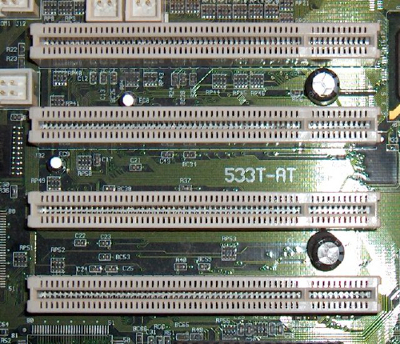
\includegraphics{Bus_pci.jpg}
\end{center}

En ambos casos (USB y PCI) suele ser de interés obtener la información de cuáles son 
los dispositivos conectados a estos puertos o buses. Convenientemente existen los 
comandos \texttt{lsusb} y \texttt{lspci}. 

Por ejemplo si conectamos un dispositivo, digamos una memoria flash (pendrive) o un 
módem 3g USB, y el sistema no realiza automáticamente las acciones que esperamos, un primer paso en la 
identificación del problema es observar si el dispositivo es reconocido o no. 

En el siguiente ejemplo, se observan tres dispositivos conectados, un teclado, 
un lector de memorias y un conector inalámbrico para mouse o teclado: 
 
\colorbox{grey}{\parbox[t]{0.95\linewidth}{ \vspace*{0.5cm} { 
{\tt
Bus 001 Device 001: ID 1d6b:0002 Linux Foundation 2.0 root hub\\
Bus 002 Device 001: ID 1d6b:0002 Linux Foundation 2.0 root hub\\
Bus 003 Device 001: ID 1d6b:0002 Linux Foundation 2.0 root hub\\
Bus 004 Device 001: ID 1d6b:0001 Linux Foundation 1.1 root hub\\
Bus 005 Device 001: ID 1d6b:0001 Linux Foundation 1.1 root hub\\
Bus 006 Device 001: ID 1d6b:0001 Linux Foundation 1.1 root hub\\
Bus 007 Device 001: ID 1d6b:0001 Linux Foundation 1.1 root hub\\
Bus 005 Device 002: ID 0430:0005 Sun Microsystems, Inc. Type 6 Keyboard\\
Bus 004 Device 002: ID 04e6:5119 SCM Microsystems, Inc. SCR3340 - ExpressCard54 Smart Card Reader\\
Bus 004 Device 003: ID 1d57:32da Xenta 2.4GHz Receiver (Keyboard and Mouse)
}
} \vspace*{0.5cm} } } 

Luego, si conectamos un módem 3g observamos un nuevo dispositivo: 

\colorbox{grey}{\parbox[t]{0.95\linewidth}{ \vspace*{0.5cm} { 
{\tt
Bus 001 Device 001: ID 1d6b:0002 Linux Foundation 2.0 root hub\\
Bus 002 Device 001: ID 1d6b:0002 Linux Foundation 2.0 root hub\\
Bus 003 Device 001: ID 1d6b:0002 Linux Foundation 2.0 root hub\\
Bus 004 Device 001: ID 1d6b:0001 Linux Foundation 1.1 root hub\\
Bus 005 Device 001: ID 1d6b:0001 Linux Foundation 1.1 root hub\\
Bus 006 Device 001: ID 1d6b:0001 Linux Foundation 1.1 root hub\\
Bus 007 Device 001: ID 1d6b:0001 Linux Foundation 1.1 root hub\\
Bus 005 Device 002: ID 0430:0005 Sun Microsystems, Inc. Type 6 Keyboard\\
Bus 004 Device 002: ID 04e6:5119 SCM Microsystems, Inc. SCR3340 - ExpressCard54 Smart Card Reader\\
Bus 004 Device 003: ID 1d57:32da Xenta 2.4GHz Receiver (Keyboard and Mouse)\\
\textbf{Bus 001 Device 005: ID 12d1:150f Huawei Technologies Co., Ltd.}
}
} \vspace*{0.5cm} } } 

En este punto sabemos, al menos que el sistema reconoce el dispositivo. 

\section{Conclusión}


\section*{Licencia}

Este texto fue creado por Miriam Tamara Lechner y se encuentra bajo 
Licencia Creative Commons Atribución-CompartirDerivadasIgual 3.0 Unported

\end{document}
